\documentclass[../thesis.tex]{subfiles}

\begin{document}

\section{Thu thập và xử lý dataset}

Chúng tôi đã chụp/trích từ video 3600 ảnh về 32 loại biển báo thường gặp trong nội đô thành phố Cần Thơ. Tập dữ liệu sau đó được xử lý, khoanh vùng và gắn nhãn trước khi chia thành 2 tập con: train và test với tỷ lệ 0.795/0.205.

\begin{figure}[!htb]
	\centering
	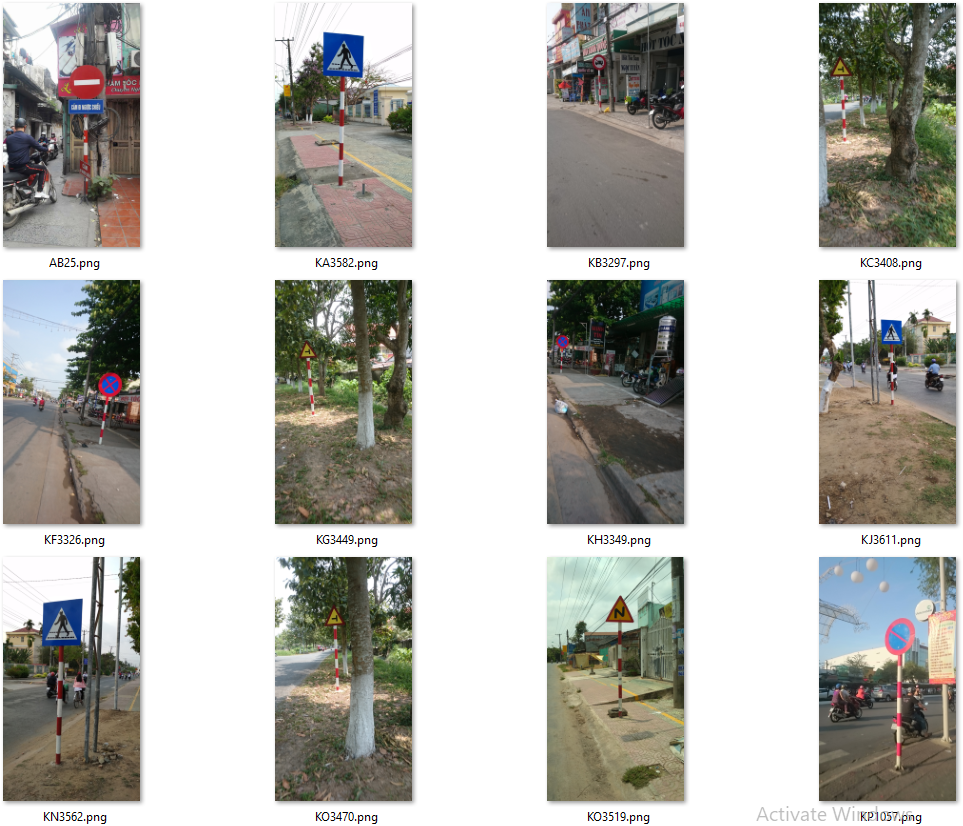
\includegraphics[width=\linewidth]{dataset.png}
	\caption{Một số mẫu dữ liệu trong dataset}\label{Fig:dataset_records}
\end{figure}

Trước tiên, chúng tôi resize chúng về cùng kích cỡ $450 \times 800$. Do các bức ảnh chứa nhiều metadata khác nhau (vì được chụp/ghi hình từ nhiều loại thiết bị) nên một phần phải trải qua thêm các bước rotate, expand, crop. Sau đó, các đối tượng biển báo nằm trong các mẫu dữ liệu được khoanh vùng và gắn nhãn bằng phần mềm mã nguồn mở LabelImg\cite{labelimg}. Mỗi bức ảnh sẽ sinh ra tương ứng một dữ liệu xml chứa các thông tin như id, path, class, bouding-box của bức ảnh đó. Giai đoạn này đòi hỏi sự kiên nhẫn và cẩn thận vì bất kỳ sai sót nào cũng có thể làm ảnh hưởng đến kết quả huấn luyện (Hình \ref{Fig:labelimg}).

\begin{figure}[!htb]
	\centering
	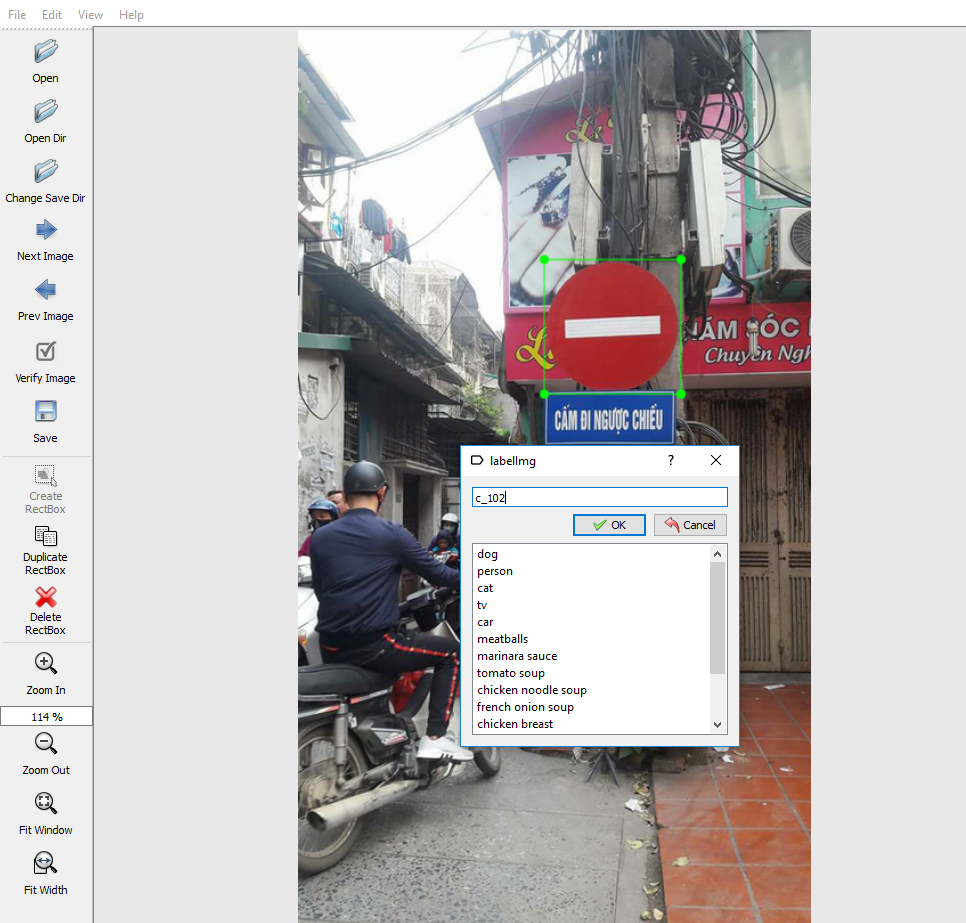
\includegraphics[width=\linewidth]{labelimg.png}
	\caption{Xử lý dữ liệu bằng phần mềm LabelImg}\label{Fig:labelimg}
\end{figure}

Tiếp đến, dataset được xáo trộn để tăng hiệu quả huấn luyện. Chúng tôi chọn ngẫu nhiên 737(20.5\%) mẫu dữ liệu làm tập test, số còn lại nằm trong tập train. Cuối cùng dữ liệu ảnh cùng với các thông tin trong các xml tương ứng sẽ được mã hóa thành định dạng tfrecord. Chương trình sử dụng định dạng này để tải lên dataset, phục vụ quá trình huấn luyện.

\begin{table}[!htb]
\begin{longtable}{| l | l | c | c |}
	\hline
	Nhãn & Mô tả & Training set & Test set\\
	\hline
	c\_102 & Cấm đi ngược chiều & 89 & 30\\
	\hline
	c\_103a & Cấm ô tô & 75 & 17\\
	\hline
	c\_106b & Cấm ô tô tải & 54 & 16\\
	\hline
	c\_107 & Cấm ô tô  khách và ô tô  tải & 98 & 32\\
	\hline
	c\_115 & Hạn chế trọng lượng xe & 240 & 70\\
	\hline
	c\_130 & Cấm dừng xe và đỗ xe & 79 & 17\\
	\hline
	c\_131a & Cấm đỗ xe & 111 & 38\\
	\hline
	nh\_201a & Chỗ ngoặt nguy hiểm vòng bên trái & 54 & 18\\
	\hline
	nh\_201b & Chỗ ngoặt nguy hiểm vòng bên phải & 57 & 19\\
	\hline
	nh\_202a & Nhiều chỗ ngoặt nguy hiểm liên tiếp & 64 & 20\\
	\hline
	nh\_202b & Nhiều chỗ ngoặt nguy hiểm liên tiếp & 70 & 9\\
	\hline
	nh\_205a & Đường giao nhau cùng cấp & 54 & 11\\
	\hline
	nh\_205b & Đường giao nhau cùng cấp & 97 & 25\\
	\hline
	nh\_205c & Đường giao nhau cùng cấp & 83 & 12\\
	\hline
	nh\_205d & Đường giao nhau cùng cấp & 90 & 14\\
	\hline
	nh\_207a & Giao nhau với đường không ưu tiên & 180 & 46\\
	\hline
	nh\_207b & Giao nhau với đường không ưu tiên & 128 & 37\\
	\hline
	nh\_207c & Giao nhau với đường không ưu tiên & 179 & 48\\
	\hline
	nh\_207d & Giao nhau với đường không ưu tiên & 60 & 15\\
	\hline
	nh\_208 & Giao nhau với đường ưu tiên & 80 & 20\\
	\hline
	nh\_209 & Giao nhau có tín hiệu đèn & 115 & 27\\
	\hline
	nh\_221b & Đường có sóng mấp mô nhân tạo & 97 & 16\\
	\hline
	nh\_224 & Đường người đi bộ cắt ngang & 161 & 37\\
	\hline
	nh\_225 & Trẻ em & 188 & 56\\
	\hline
	nh\_233 & Nguy hiểm khác & 56 & 16\\
	\hline
	hl\_303 & Nơi giao nhau chạy theo vòng xuyến & 79 & 18\\
	\hline
	cd\_423a & Đường người đi bộ sang ngang & 77 & 15\\
	\hline
	cd\_423b & Đường người đi bộ sang ngang & 80 & 15\\
	\hline
	cd\_425 & Bệnh viện & 74 & 31\\
	\hline
	cd\_428 & Trạm cung cấp xăng dầu & 70 & 14\\
	\hline
	cd\_434 & Bến xe buýt & 114 & 39\\
	\hline
	cd\_443 & Chợ & 63 & 10\\
	\hline
	\multicolumn{2}{|c|}{\textbf{Tổng}} & \textbf{3116} & \textbf{808}\\
	\hline
\end{longtable}
\caption{Thông tin về tập dữ liệu}
\label{Table:datset}
\end{table}
\end{document}